% arara: xelatex: {synctex: true}
% arara: indent: {overwrite: yes}
\documentclass[]{IMTexam}

\usepackage[enums]{IMTtikz}

\givecredits
\author{Isabella B.}
\USPN{11810773}
\date{}
\lecture{Física I} % disciplina
\lcode{4302111}
\hwtype{Resolução} % o que é
\examname{Provinha III} % prova

\begin{document}

\maketitle

\begin{questions}

	\question \label{ques:q1}
	Considere um corpo de massa $ M $ que no referencial $ S $ têm velocidade $\vec{u}$, posição $\vec{x}$ e energia $ E= \dfrac{|\vec{P}|^{2}}{2M} + U_{int}(\vec{x}) $, onde $ \vec{P} = M\vec{u} $ é o seu momento total. Suponha que a energia potencial de interação $ U_{int}(\vec{x}) $ seja invariante por transformações de Galileu, isto é, $ U_{int}(\vec{x}+\vec{V}t)=U_{int}(\vec{x}) $ para qualquer velocidade $\vec{V}$ e tempo $ t $. Com isso em mente, responda as seguintes questões:

	\begin{parts}
		\part \label{part:q1a} Em um referencial $ S' $, se movendo com velocidade $ -\vec{V} $ em relação a $ S $, ache a velocidade $ \vec{u'} $ do corpo e prove que sua energia é dada por $ E'=E+\sfrac{1}{2}M|\vec{V}|^{2}+\vec{V}\cdot\vec{P} $.

		(Ainda que não tenha derivado os resultados acima, é permitido utilizá-los nos itens a seguir)

		\begin{solution}
			\begin{multi}
				Dado $ \dot{\vec{x}}=\vec{u} $, sabemos, por transformações de Galileu, que
				\begin{gather}
					\vec{u-u'=-V}\implies\vec{u'}=\vec{u}+\vec{V} \label{eq:q1aS1}\\ \intertext{multiplicando a eq. \ref{eq:q1aS1} por $ M $}
					\vec{P'}=\vec{P}+M\vec{V}\label{eq:q1aS2}\\ \intertext{integrando a eq. \ref{eq:q1aS1} com respeito a $ t $}
					\vec{x'}=\vec{x}+\vec{V}t\label{eq:q1aS3}
				\end{gather}
				\nach
				\centering
				\begin{tikzpicture}
					\coordinate (Si) at (0,0);
					\draw[->] (Si)++(-0.5,0) -- +(2,0);
					\draw[->] (Si)++(0,-0.5) -- +(0,2);
					\node[below left] at (Si) {$ S $};

					\coordinate (Sd) at (3,2);
					\draw[->] (Sd)++(-0.5,0) -- +(2,0);
					\draw[->] (Sd)++(0,-0.5) -- +(0,2);
					\node[below right] at (Sd) {$ S' $};

					\coordinate (obj) at (1,3);
					\draw[-Latex] (Si) -- node[above left] {$ \vec{u} $} (obj);
					\draw[-Latex] (Sd) -- node[above right] {$ \vec{u'} $}(obj);
					\draw[-Latex] (Si) -- node[below right] {$ -\vec{V} $} (Sd);

					\filldraw (obj) circle (2pt) node[above] {Corpo};
				\end{tikzpicture}
			\end{multi}


			Tomando $ E'=\dfrac{|\vec{P'}|^{2}}{2M} + U_{int}(\vec{x'}) $ (dada no enunciado) e substituindo as equações \ref{eq:q1aS2} e \ref{eq:q1aS3}, teremos:

			\begin{align*}
				E' & =\dfrac{|\vec{P}+M\vec{V}|^{2}}{2M} + U_{int}(\vec{x}+\vec{V}t)                                                                      \\
				   & =\dfrac{\del{\sqrt{(\vec{P}+M\vec{V})(\vec{P}+M\vec{V})}}^{2}}{2M} + U_{int}(\vec{x})                                                \\
				   & =\dfrac{\envert{\vec{P}\cdot\vec{P}+(M\vec{V})\cdot\vec{P}+\vec{P}\cdot(M\vec{V})+(M\vec{V})\cdot(M\vec{V})}}{2M} + U_{int}(\vec{x}) \\
				   & =\dfrac{\envert{\vec{P}\cdot\vec{P}+M^{2}\vec{V}\cdot\vec{V}+2M\vec{V}\cdot\vec{P}}}{2M} + U_{int}(\vec{x})
			\end{align*}
			sabendo que $ \vec{P}\cdot\vec{P}=|\vec{P}|^{2}>0 $ e $ \vec{V}\cdot\vec{V}=|\vec{P}|^{2}>0 $, e assumindo $ M>0 $, temos
			\begin{align*}
				E' & =\dfrac{|\vec{P}|^{2}+M^{2}|\vec{V}|^{2}+2M\vec{V}\cdot\vec{P}}{2M} + U_{int}(\vec{x})                                                                                 \\
				   & =\underbrace{\dfrac{|\vec{P}|^{2}}{2M}+ U_{int}(\vec{x})}_{=E} + \dfrac{M^{\cancel{2}}|\vec{V}|^{2}}{2\cancel{M}}+ \dfrac{\cancel{2M}\vec{V}\cdot\vec{P}}{\cancel{2M}} \\[1ex]
				   & =E+\dfrac{M|\vec{V}|^{2}}{2}+\vec{V}\cdot\vec{P}
			\end{align*}

			\hfill\qedsymbol
		\end{solution}

		\clearpage

		\part \label{part:q1b} Fixados $ |\vec{V}| $ e $ |\vec{P}| $, prove que o mínimo de $ \vec{V}\cdot\vec{P} $ é $ -|\vec{V}||\vec{P}| $.

		(Dica: Interprete $ \vec{V}\cdot\vec{P} $ geometricamente.)

		\begin{solution}
			\begin{multi}[3]
				Dados os vetores $ \vec{V} $ e $ \vec{P} $, que possuem módulos constantes, respectivamente $ |\vec{V}| $ e $ |\vec{P}| $, sendo $ \vec{V}\cdot\vec{P} $ a multiplicação da projeção ortogonal de $ \vec{V} $ em $ \vec{P} $ pelo módulo de $ \vec{P} $ (ou vice-versa, pois $ \vec{V}\cdot\vec{P} = \vec{P}\cdot\vec{V} $), pela equação $ \vec{V}\cdot\vec{P}=|\vec{V}||\vec{P}|\cos\theta $, onde $\theta$ é o ângulo entre eles, temos que o valor mínimo de $ \vec{V}\cdot\vec{P}=-|\vec{V}||\vec{P}| $, pois $ -1\leqslant\cos\theta\leqslant1 $ sendo, portanto, $ \cos\ang{180}=-1 $ seu valor mínimo, na situação onde $ \vec{V} $ e $ \vec{P} $ apontam em direções opostas.
				\nach
				\centering
				\begin{tikzpicture}
					\coordinate (O) at (0,0);
					\draw[->] (-0.5,0) -- +(3,0);
					\draw[->] (0,-0.5) -- +(0,3);

					\coordinate (V) at (1,2);
					\coordinate (P) at (2,1);

					\draw[-Latex] (O) -- node[above left] {$ \vec{V} $} (V);
					\draw[-Latex] (O) -- node[above right, at end] {$ \vec{P} $} (P);
					\draw[dashed] (V) -- ($ (O)!(V)!(P) $) coordinate (proj);
					\draw[decorate,decoration={brace,amplitude=5pt,mirror,raise=2pt}] (O) -- node[below right=5pt,rotate=25] {$ |\vec{V}|\cos\theta $} (proj);

					\dotMarkRightAngle[size=5pt](V,proj,O)

					\pic[draw=black, angle radius=15pt,angle eccentricity=1,"$ \theta $" {xshift=4pt,yshift=4pt}] {angle=P--O--V};

					%			\node[below left] at (Si) {$ S $};
				\end{tikzpicture}

				Caso qualquer
				\nach

				\centering
				\begin{tikzpicture}
					\coordinate (O) at (0,0);
					\draw[->] (-2.5,0) -- (2.5,0);
					\draw[->] (0,-1.5) -- (0,1.5);

					\coordinate (V) at (2,1);
					\coordinate (P) at (-2,-1);

					\draw[-Latex] (O) -- node[above] {$ \vec{V} $} (V);
					\draw[-Latex] (O) -- node[below=2pt] {$ \vec{P} $} (P);
					%			\draw[dashed] (V) -- ($ (O)!(V)!(P) $) coordinate (proj);
					%			\draw[decorate,decoration={brace,amplitude=5pt,mirror,raise=2pt}] (O) -- node[below right=5pt,rotate=25] {$ |\vec{V}|\cos\theta $} (proj);

					%			\dotMarkRightAngle[size=5pt](V,proj,O)

					\pic[draw=black, angle radius=10pt,angle eccentricity=1,"$ \theta=\ang{180} $" {rotate=25,xshift=-10pt,yshift=8pt}] {angle=V--O--P};

					%			\node[below left] at (Si) {$ S $};
				\end{tikzpicture}

				Caso mínimo
			\end{multi}

			\hfill\qedsymbol
		\end{solution}
	\end{parts}

	\medskip

	\question \label{ques:q2}
	Agora estamos em posição de entender o argumento de Landau. Para isso considere a Figura \ref{fig:fig1}:

	\begin{figure}[H]
		\centering
		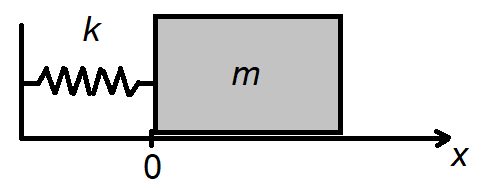
\includegraphics[width=0.5\linewidth]{screenshot001}
		\caption{Diagramas das diferentes situações do fluido retratadas no texto.}
		\label{fig:fig1}
	\end{figure}

	Landau imaginou um fluido de massa $ M $ e velocidade $\vec{V}$ (veja a Figura \ref{fig:fig1}(a)) escoando em um tubo estreito. Para um fluido normal, com viscosidade, suas interações com o tubo seriam a causa primária do atrito viscoso e da dissipação de energia que as partículas no fluido sofrem.

	Ele considerou que o mecanismo para a viscosidade seria a criação de excitações no fluido que se propagariam com momento $\vec{p}$ e relação de dispersão $\epsilon(|\vec{p}|)$\footnote{Lembre-se novamente de que aqui estamos assumindo uma forma geral dessa relação e não necessariamente que seja igual à $ |\vec{p}|^{2}/2m $}, por conta da interação com o tubo. As excitações não devem ser entendidas como partículas no sentido usual, pois elas são a combinação de complexos movimentos ocorrendo no fluido (exemplos serão dados mais a frente).

	\begin{parts}
		\part \label{part:q2a} Considere a situação da Figura \ref{fig:fig1}(b). Ela representa a visão de um observador no \textbf{referencial de repouso} $ S $ do fluido. Suponha que, sem excitação, a energia do fluido nesse referencial seja $ E_0 $, chamada \textit{energia do estado fundamental}. Com a adição de uma excitação de energia $ \epsilon(|\vec{p}|) $ e momento $\vec{p}$, qual será a nova energia $ E $ e o novo momento $\vec{P}$ do fluido nesse mesmo referencial?

		\begin{solution}
			$ E $ e $ \vec{P} $ devem ser $ E=E_0+\epsilon(|\vec{p}|) $ e $ \vec{P}=\vec{p} $, respectivamente.
		\end{solution}

		\part Com base no exercício \ref{ques:q1}(\ref{part:q1a}), faça uma transformação de Galileu para referencial de laboratório $ S' $, no qual o fluido se move com velocidade $\vec{V}$ (veja a Figura \ref{fig:fig1}(d)), e encontre o momento $\vec{P'}$ e energia $ E' $ do fluido nesse referencial.

		(Ainda que não seja necessário, podemos assumir que $ |\vec{p}|^{2}/2M \ll E' $ para simplificar as contas, pois se espera que o momento da excitação seja muito menor do que o momento do fluido $ M\vec{V} $.)

		\begin{solution}
			\begin{multi}
				Pela transformação de Galileu, enquanto a velocidade do fluido no referencial anterior seria meramente $ \vec{u}=\vec{0} $, agora será $ \vec{u'}=\vec{V} $, e, portanto, pelos resultados da questão \ref{ques:q1}(\ref{part:q1a}) a energia $ E' $ no novo referencial será
				\begin{gather}
					E'=E+\dfrac{M|\vec{V}|^{2}}{2}+\vec{V}\cdot\vec{P} \label{eq:q2bS1}\\
					\intertext{e}
					\vec{P'}=\vec{P}+M\vec{V} \label{eq:q2bS2}
				\end{gather}
				\nach
				\centering
				\begin{tikzpicture}
					\coordinate (Si) at (0,0);
					\draw[->] (Si)++(-0.5,0) -- +(2,0);
					\draw[->] (Si)++(0,-0.5) -- +(0,2);
					\node[below right] at (Si) {$ S' $ (laboratório)};

					\coordinate (Sd) at (3,2);
					\draw[->] (Sd)++(-0.5,0) -- +(2,0);
					\draw[->] (Sd)++(0,-0.5) -- +(0,2);
					\node[below right] at (Sd) {$ S $ (fluido)};

					\coordinate (obj) at (1,3);
					%			\draw[-Latex] (Si) -- node[above left] {$ \vec{u} $} (obj);
					%			\draw[-Latex] (Sd) -- node[above right] {$ \vec{u'} $}(obj);
					\draw[-Latex] (Si) -- node[below right] {$ \vec{V} $} (Sd);

					%			\filldraw (obj) circle (2pt) node[above] {Corpo};
				\end{tikzpicture}
			\end{multi}

		\end{solution}

		\part Qual seria a energia $\tilde{E}$ e o momento $\tilde{\vec{P}}$ do fluido \textbf{sem excitação}, no referencial do laboratório? Prove que a diferença de energia é dada por $ \Delta E=E'-\tilde{E}=\epsilon(|\vec{p}|)+\vec{p}\cdot\vec{V} $.

		(Dica: Não é necessário refazer todas as contas. Tente adaptar o item anterior, porém não esqueça de dar justificativas)

		(Ainda que não tenha derivado os resultados acima, é permitido utilizá-los nos itens a seguir)

		Se o custo para criar a excitação $ \Delta E $ for menor do que zero, então as excitações serão criadas espontaneamente. Portanto, para que o fluido perca energia pela dissipação induzida por essas excitações, é necessário e suficiente que $ \Delta E < 0 $.

		\begin{solution}
			Considerando o mesmo fluido sob transformação de Galileu, porém sem a excitação da questão \ref{ques:q2}(\ref{part:q2a}). Adotando momento inicial nulo, teríamos
			\begin{gather}
				\tilde{E}=E_0+\dfrac{M|\vec{V}|^{2}}{2}\label{eq:q2cS1}\\
				\intertext{e}
				\tilde{\vec{P}}=M\vec{V}\label{eq:q2cS2}
			\end{gather}
			Fazendo $ \Delta E=E'-\tilde{E} $, temos
			\begin{align*}
				\Delta E=E'-\tilde{E} & =\del{E+\dfrac{M|\vec{V}|^{2}}{2}+\vec{V}\cdot\vec{P}}-\del{E_0+\dfrac{M|\vec{V}|^{2}}{2}}                                               \\
				                      & =\cancel{E_0}+\epsilon(|\vec{p}|)+\cancel{\dfrac{M|\vec{V}|^{2}}{2}}+\vec{V}\cdot\vec{p}-\cancel{E_0}-\cancel{\dfrac{M|\vec{V}|^{2}}{2}}
			\end{align*}
			pela simetria do produto escalar
			\begin{equation}
				\Delta E=\epsilon(|\vec{p}|)+\vec{p}\cdot\vec{V}\label{eq:q2cS3}
			\end{equation}

			\hfill\qedsymbol
		\end{solution}

		\part Fixados $ |\vec{p}| $ e $ |\vec{V}| $, só pode haver $ \Delta E < 0 $ se o seu mínimo for menor que zero também. Usando o item \ref{ques:q1}(\ref{part:q1b}), prove que o mínimo de $ \Delta E $ nessas condições é $ \epsilon(|\vec{p}|)-|\vec{p}||\vec{V}| $. Prove então que só pode haver $ \Delta E<0 $ se $ |\vec{V}|>\epsilon(|\vec{p}|)/|\vec{p}| $, com $ \vec{p}\neq\vec{0} $.

		No caso oposto, ou seja, supondo que tenhamos $ \Delta E>0 $, é necessário dispêndio de energia para criar \textbf{qualquer excitação}. Logo um fluido no regime de velocidade
		\begin{equation}\label{eq:eq1}
			|\vec{V}|<\min_{\vec{p}\neq\vec{0}}\dfrac{\epsilon(|\vec{p}|)}{|\vec{p}|}
		\end{equation}
		não apresentaria viscosidade, sendo então um \textbf{superfluido}!

		\begin{solution}
			Pelo item \ref{ques:q1}(\ref{part:q1b}), temos
			\[ \min\vec{p}\cdot\vec{V}=-|\vec{p}||\vec{V}| \]
			dado $ |\vec{p}| $ fixado, admitimos $ \epsilon(|\vec{p}|) $ fixado também, e daí segue, da eq. \ref{eq:q2cS3}
			\begin{equation}
				\min\Delta E=\epsilon(|\vec{p}|)-|\vec{p}||\vec{V}| \label{eq:q2dS1}
			\end{equation}
			e para que a eq. \ref{eq:q2dS1} seja menor que zero, precisamos que
			\begin{align*}
				\epsilon(|\vec{p}|) & <|\vec{p}||\vec{V}|                     \\
				\intertext{assumindo $ \vec{p}\neq\vec{0} $}
				|\vec{V}|           & >\dfrac{\epsilon(|\vec{p}|)}{|\vec{p}|}
			\end{align*}

			\hfill\qedsymbol
		\end{solution}

		\part \label{part:q2e} Imagine que as excitações sejam ondas de som, cuja energia é proporcional ao momento:
		\begin{equation}\label{eq:eq2}
			\epsilon(|\vec{p}|)=v_s|\vec{p}|
		\end{equation}
		onde $ v_s $ é a velocidade do som. Usando a equação \ref{eq:eq1}, mostre que existe uma velocidade crítica $ v_c $, abaixo da qual ocorre superfluidez, e que seu valor é $ v_c = v_s $. Excitações desse tipo são chamada fônons.

		\begin{solution}
			Sendo $ v_c $ a velocidade crítica, estabelecida na equação \ref{eq:eq1}, temos
			\[ |\vec{V}|<v_c=\min_{\vec{p}\neq\vec{0}}\dfrac{\epsilon(|\vec{p}|)}{|\vec{p}|} \]

			Pela eq. \ref{eq:eq2}, temos
			\[ \epsilon(|\vec{p}|)=v_s|\vec{p}|\overset{\vec{p}\neq\vec{0}}{\implies} v_s=\dfrac{\epsilon(|\vec{p}|)}{|\vec{p}|}\quad\text{(constante)} \]
			daí, tiramos
			\[ v_c=v_s \]

			\hfill\qedsymbol
		\end{solution}

		\clearpage

		\part No caso “normal” de excitações massivas do tipo $ \epsilon(|\vec{p}|)= \dfrac{|\vec{p}|^{2}}{2m} $, mostre que a velocidade crítica é $ v_c = 0 $, isto é, \textbf{não ocorre estado superfluido}.

		\begin{solution}
			Da equação \ref{eq:eq1}, temos:
			\begin{align*}
				|\vec{V}| & <\min_{\vec{p}\neq\vec{0}}\dfrac{\epsilon(|\vec{p}|)}{|\vec{p}|}=v_c \\ \intertext{substituindo $ \epsilon(|\vec{p}|)= |\vec{p}|^{2}/2m $}
				v_c       & =\min_{\vec{p}\neq\vec{0}}\dfrac{|\vec{p}|^{2}/2m}{|\vec{p}|}        \\
				          & =\min_{\vec{p}\neq\vec{0}}\dfrac{|\vec{p}|}{2m}                      \\ \intertext{como $ \vec{p}\neq\vec{0} $, devemos tomar o limite $ |\vec{p}|\to0 $}
				v_c       & =\lim\limits_{|\vec{p}|\to0}\dfrac{|\vec{p}|}{2m}=0
			\end{align*}

			\hfill\qedsymbol
		\end{solution}

		\bigskip

		\part \label{part:q2g} Existem excitações chamadas rótons que possuem relação de dispersão dada por
		\begin{equation}\label{eq:eq3}
			\epsilon(|\vec{p}|)=\Delta+\dfrac{(|\vec{p}|-p_0)^{2}}{2\mu}\, ,
		\end{equation}
		onde $ p_0,\mu $ e $ \Delta $ são constantes independentes de $\vec{p}$. Determine a velocidade crítica $ v_c $ nesse caso.

		%	\paragraph{Dica:} O software Mathematica pode ser utilizado para fazer as substituições algébricas e cálculos nessa questão. Não é estritamente necessário, porém, alivia o trabalho braçal. Algumas funções que podem ajudar são \verb|FullSimplify| e o \verb|ReplaceAll| (é uma função muito utilizada e pode ser abreviada por \verb|/.|). Na página do curso tem um tutorial para instalação e sobre as funções básicas. Escolha valores de $ \Delta,p_0 $ e $ \mu $ e utilize seu resultado para construir o gráfico da parábola e da reta associada a velocidade crítica e confirme que, de fato eles se tangenciam.
		%	
		%	\paragraph{Observação:} O aluno que fizer as contas utilizando o Mathematica deve enviar o arquivo \verb|.nb| para o e-mail do monitor correspondente.

		\begin{solution}
			Supondo $ \mu>0 $, sem perda de generalidade, temos que \[ \epsilon(|\vec{p}|)=a|\vec{p}|^{2}+b|\vec{p}|+c \] com $ a>0 $.
			Disso, concluímos que seu valor mínimo se dá quando \[ \dod{}{|\vec{p}|}\sbr{\epsilon(|\vec{p}|)}=0. \]
			Sendo assim, para algumas relações de dispersão quadráticas $ \epsilon(|\vec{p}|) $ bem comportadas, o valor da reta $ v(|\vec{p}|) $ passando por $ (0,0) $ e tangenciando $ \epsilon(|\vec{p}|) $ será solução de $ v_c=\epsilon(|\vec{p}|)/|\vec{p}| $.
			Podemos analisar o comportamento dessa reta tangente $ \epsilon(|\vec{p}|) $ no Mathematica (arquivo enviado por e-mail).
			%\begin{mmaCell}[functionlocal={pvfun,dispfun},
			%	pattern={p0_,p0,p_,p}]{Input}
			%dispfun[\mmaPat{Δ_}, \mmaPat{\textmu_}, p0_, p_ := \mmaPat{Δ} + (p - p0)^2/(2 \mmaPat{\textmu})
			%\end{mmaCell}
			%	daí, devemos encontrar o coeficiente angular $ m $ da reta fazendo:
			%\begin{mmaCell}[moredefined={pvfun,dispfun}]{Input}
			%FullSimplify[(dispfun[Delta, Mu, p0, p] - 0)/(p - 0)]
			%\end{mmaCell}
			%
			%\begin{mmaCell}[moredefined={pvfun,dispfun}]{Input}
			%FullSimplify[D[dispfun[Delta, Mu, p0, p], p]]
			%\end{mmaCell}
			%
			%\begin{mmaCell}[moredefined={pvfun,dispfun}]{Input}
			%FullSimplify[Solve[(Delta + (p - p0)^2/(2 Mu))/p == (p - p0)/Mu, p]]
			%\end{mmaCell}
			%
			%\begin{mmaCell}[moredefined={pvfun,dispfun}]{Input}
			%FullSimplify[(p - p0)/\[Mu] /. 
			%	p -> Sqrt[p0^2 + 2 \[CapitalDelta] \[Mu]]]
			%\end{mmaCell}
			%
			%\begin{mmaCell}[moredefined={pvfun,dispfun}]{Input}
			%	FullSimplify[(dispfun[Delta, Mu, p0, p] - 0)/(p - 0)]
			%\end{mmaCell}
			%	
			%\begin{mmaCell}[functionlocal={pvfun,dispfun},
			%	pattern={p0_,p0,p_,p}]{Input}
			%	dispfun[\mmaPat{Δ_}, \mmaPat{\textmu_}, p0_, p_ := \mmaPat{Δ} + (p - p0)^2/(2 \mmaPat{\textmu})
			%\end{mmaCell}
			%\begin{mmaCell}[
			%	moredefined={Manipulate,pvfun,dispfun}]{Code}
			%Manipulate[Show[
			%	{Plot[{dispfun[Delta, mu, p0, modp]}, {modp, -5, 20}, 
			%		PlotStyle -> Red],
			%		Plot[{pvfun[modv, modp]}, {modp, -5, 20}, PlotStyle -> Blue]}, 
			%	PlotRange -> All, AxesOrigin -> {0, 0}],
			%	{Delta, -10, 10}, {mu, -10, 10}, {p0, -10, 10}, {modv, -10, 10}
			%]
			%\end{mmaCell}
			%Fazendo
			%\begin{mmaCell}[moredefined={Manipulate,pvfun,dispfun}]{Input}
			%Minimize[\{dispfun[Delta, mu, p0, modp], modp >= 0, mu > 0\}, \{modp\}]
			%\end{mmaCell}




			%		Usando a função \verb|Minimize| no Mathematica e assumindo que $ |\vec{p}|>0 $, temos:
			%		\[ \left\lbrace 
			%		\begin{array}{cc}
			%			p_0/\mu & \mu>0 \land \dfrac{p_0^{2}}{\mu}+2\Delta=0\\
			%			\dfrac{p_0+\sqrt{p_0^{2}+2\Delta\mu}}{\mu} & \mu>0 \land p_0^{2}+2\Delta>0\\
			%			-\infty & \del{\mu>0\land p_0^{2}+2\Delta<0}\lor\mu<0\\[1ex]
			%			\infty & \text{Verdadeiro}
			%		\end{array}, 
			%		|\vec{p}|\to 
			%		\left\lbrace 
			%		\begin{array}{cc}
			%			\sqrt{p_0^{2}+2\Delta\mu}&\mu>0\land p_0^{2}+2\Delta\mu>0\\[1ex]
			%			\text{Indeterminação}&\text{Verdadeiro}
			%		\end{array}\right\rbrace 
			%		\right\rbrace  \]
		\end{solution}

		%	\bigskip

		\clearpage

		\part \label{part:q2h} Represente graficamente na Figura \ref{fig:fig2} a velocidade crítica para a relação de dispersão representada. Justifique.

		(Dica: Qual o significado geométrico da equação \ref{eq:eq1}?)

		\begin{solution}
			\begin{multi}
				Pelo mesmo raciocínio do item anterior, podemos notar que $ v_c $ corresponde ao ponto onde a reta tangente à relação de dispersão (e que passa pela origem) tem coeficiente angular mínimo e, portanto, será a reta ao lado.

				\nach

				\begin{figure}[H]
					\centering
					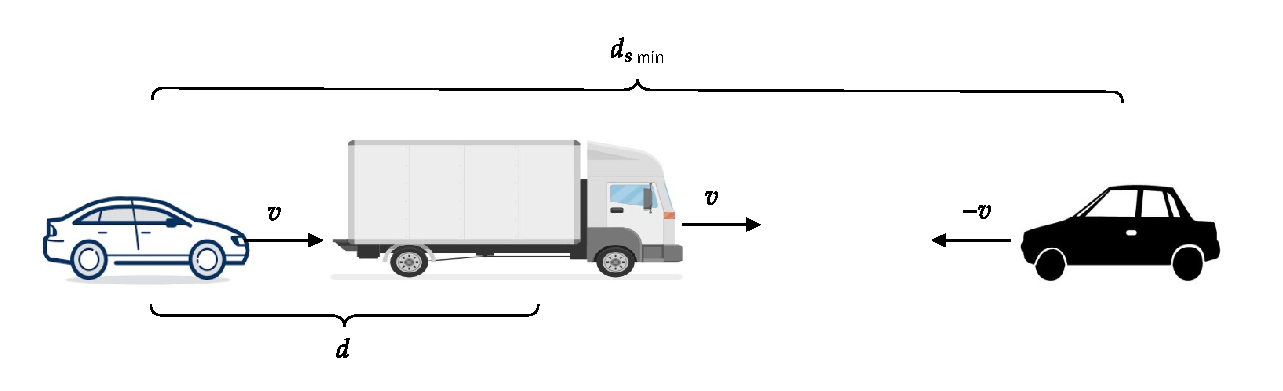
\includegraphics[width=0.5\linewidth]{diagram1}
					\caption{Relação de dispersão}
					\label{fig:fig2}
				\end{figure}
			\end{multi}

			%	\paragraph{Nota:} Conferindo pelos valores dados no gráfico, o primeiro ponto de derivada zero tem $ v\approx14/\num{1.1}\approx\num{12.72}LT^{-1} $, o terceiro tem $ v\approx17/\num{2.7}\approx\num{6.3}LT^{-1} $ e o segundo ($ v_c $) tem $ v\approx9/\num{1.9}\approx\num{4.3}LT^{-1}=v_c $.
		\end{solution}

		%	\clearpage

		\part A partir dos itens \ref{ques:q2}(\ref{part:q2e}) e \ref{ques:q2}(\ref{part:q2g}), indique na Figura \ref{fig:fig3} a região aproximada correspondente a excitações de fônons e a de rótons. Justifique sua escolha. Qual delas é a mais importante para a velocidade crítica e por quê?

		\begin{solution}
			\begin{multi}
				Considerando a região em torno do ponto marcado na resolução do item \ref{ques:q2}(\ref{part:q2h}) é semelhante a uma parábola com concavidade para cima e que está perto da origem, a região grifada de \textcolor{red}{vermelho} deve ser uma boa aproximação para a excitação dos rótons.

				\medskip

				Já as excitações dos fônons, que podem ser descritas como retas com coeficiente angular alto e próximas da origem, podem ser aproximadas pela região grifada em \textcolor{blue}{azul}.

				\medskip

				Sendo as excitações dos rótons mais pontuais, são mais importantes como demarcação da velocidade crítica (as excitações dos fônons podem variar mais de valor crítico).

				\nach

				\begin{figure}[H]
					\centering
					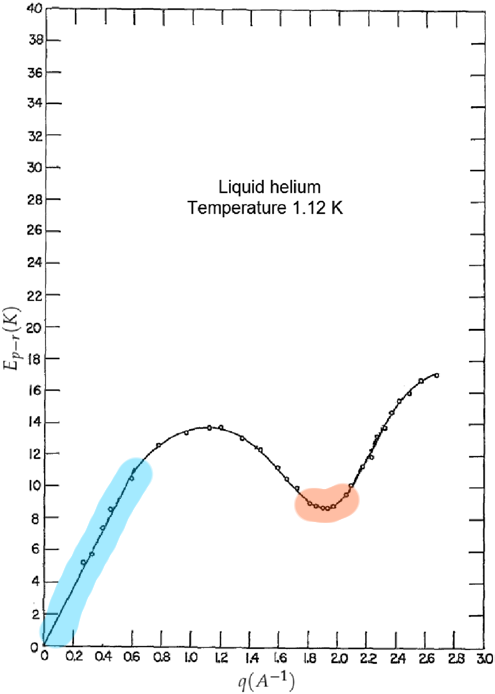
\includegraphics[width=0.6\linewidth]{diagram3}
					\caption{Relação de dispersão}
					\label{fig:fig3}
				\end{figure}
			\end{multi}
		\end{solution}

	\end{parts}

\end{questions}
\end{document}
